\documentclass{article}

% NeurIPS 2023 style file (the 2024/2025 copies were not downloadable at the time of writing).
% [preprint] gives the arXiv look; replace with [final] for a camera-ready, or no option for review.
\usepackage[preprint]{neurips_2023}

\usepackage[utf8]{inputenc}
\usepackage{hyperref}
\usepackage{url}
\usepackage{booktabs}
\usepackage{amsfonts}
\usepackage{microtype}
\usepackage{xcolor}
\usepackage{graphicx}
\usepackage{listings}
\usepackage{caption}
\usepackage{subcaption}

\lstset{basicstyle=\ttfamily\scriptsize,breaklines=true,columns=fullflexible,frame=single}
\newcommand{\todo}[1]{\textcolor{red}{[TODO: #1]}}
\newcommand{\Es}{\ensuremath{\mathbb{E}[s]}}

\title{Tactile FLORA: Fingertip Force as Text Improves a Vision-Language Reward Model's Grasp Judgments}

\author{%
  Oren Gershony \\
  Triton Droids, UC San Diego \\
  \texttt{ogershony@ucsd.edu} \\
  \And
  Aaryan Patel \\
  Triton Droids, UC San Diego \\
  \texttt{aap025@ucsd.edu} \\
  \And
  Kenan Blair \\
  Triton Droids, UC San Diego \\
  \texttt{keblair@ucsd.edu} \\
  \And
  Parth Trivedi \\
  Triton Droids, UC San Diego \\
  \texttt{patrivedi@ucsd.edu} \\
}

\begin{document}

\maketitle

\begin{abstract}
Vision-language reward models judge whether a robot completed a task from video alone, yet the
outcome of a grasp is often decided at the fingertips, where a camera cannot see whether contact
was made, held, or lost. We add a fingertip-force channel to NVIDIA's FLORA-Rewarder (a
Qwen3.5-27B video reward model) without changing its architecture: the force stream is normalized,
rendered as a short text block with a label-free summary line, and placed in the prompt after the
video. Fine-tuning with LoRA on 350 grasp clips from the HRDexDB Inspire-hand dataset, we compare
the tactile model with the released model and with a matched fine-tune on the same clips and
settings but with the force block omitted. On 251 held-out clips over 32 unseen objects the tactile
model reaches 79.3\% accuracy and 0.873 AUROC against 76.5\% / 0.830 for the video-only fine-tune
and 66.5\% / 0.600 for the released model; the ranking gain over the matched control is
$+0.043$ AUROC (object-level bootstrap 95\% interval $+0.001$ to $+0.080$, $p \approx 0.02$).
Shuffling the force blocks between clips removes the gain ($p = 0.009$) and blanking the video
leaves only the force's own moderate signal (AUROC 0.775), so the model reads both channels. The
gain concentrates on the clips where the video-only model is unsure. On ten live rollouts of an
ACT policy on a Rethink Baxter with home-built force-sensing fingertips, evaluated zero-shot, the
force block takes the ranking of the two successful grasps from below chance (AUROC 0.31 for the
video-only fine-tune, 0.38 for the released model) to perfect (1.0), while shuffled force gives
0.25 and removed force 0.44. Force rendered as text is a cheap, inspectable way to give a video
reward model the contact information it lacks.
\end{abstract}

\section{Introduction}

Reward models that watch a video and score whether a manipulation task succeeded are becoming the
labelling engine behind robot learning at scale: they rank rollouts, filter demonstrations and
supply rewards for policy improvement. FLORA~\cite{flora2026} is a recent example: a family of
fine-tuned Qwen3.5 vision-language models whose reward member takes a multi-camera clip and a task
instruction and answers with an outcome score from 1 to 5. It is vision-only.

Grasping is the case where vision-only judgment is weakest. The decisive events of a grasp, whether
the fingers actually closed on the object, how firmly they hold it, whether the hold is slipping
and when contact ends, happen at the fingertips, occluded by the hand itself, and leave few
pixels in a camera view. A loaded gripper lifting an object and an empty gripper lifting nothing
can look identical from a head camera. Fingertip force sensors see exactly these events, and they
are cheap. Our hypothesis is that \emph{fingertip force reveals contact failures that RGB misses or
sees late}, and that a video reward model can be taught to use it.

The question is how to give a large vision-language model a new sensor without retraining it.
Learned encoders and adapter tokens are possible but opaque and data-hungry. We take the
simplest route: render the force as text. The force stream is resampled to the frames the model
already samples, normalized so that 0 is free space and 1 is a typical grasp, and written as one
line per frame with a label-free summary line at the top. The block enters the prompt after the
video, with one sentence explaining its columns. The model is then fine-tuned with LoRA on
outcome-labelled clips. Everything else, the released weights, prompts, frame sampling and answer
format, stays as released.

Our contributions are:
\begin{itemize}
  \item A force-as-text representation for a video reward model, with the normalization,
  summary statistics and a small force-only classifier probability that make the signal legible
  to the language model (Section~\ref{sec:method}).
  \item A controlled evaluation on object-disjoint held-out splits of HRDexDB~\cite{hrdexdb2026},
  with two controls that isolate the force contribution: a matched fine-tune without force, and
  a shuffled-force ablation (Section~\ref{sec:results}).
  \item A zero-shot transfer test on a different embodiment: a Rethink Baxter with force-sensing
  fingertips we built, running a learned policy, where the force block decides the ranking of
  successes over failures (Section~\ref{sec:baxter-results}).
  \item An account of what went wrong first. A naive force rendering produced no gain; an audit of
  the block the model actually read found it nearly uninformative, and correcting the
  representation, not the model, produced the result (Section~\ref{sec:process}).
\end{itemize}

\section{Related work}

\paragraph{Vision-language reward models.} FLORA~\cite{flora2026} fine-tunes Qwen3.5 models into
a segmenter, a captioner and a reward model that scores task outcome and dense execution quality
from video; related video reward models and benchmarks include RoboReward~\cite{lee2026roboreward} and
Robometer~\cite{liang2026robometer}, and vision-language models have been used as success
detectors since SuccessVQA~\cite{du2023successvqa}. These models are vision-only. We keep FLORA's reward model and add one
sensor channel to its prompt.

\paragraph{Tactile sensing for grasp outcome.} Fingertip force has long been used to detect
grasp success, slip and contact loss~\cite{veiga2015slip,yuan2017gelsight,calandra2017feeling},
and recent datasets pair tactile streams with manipulation video~\cite{hrdexdb2026}. Our
force-only probes agree with that literature: force statistics alone separate HRDexDB grasp
outcomes at AUROC 0.76 to 0.80, a real but moderate signal, weaker than video alone (0.90).

\paragraph{Sensor data as text for language models.} Serializing time series and sensor readings
as text for a language model is a known technique~\cite{gruver2023llmtime,jin2024timellm,xu2024penetrative}. Our contribution is not the idea but the demonstration that a video reward model can learn
to combine such a block with video under LoRA, and the controls that show it does.

\section{Method}
\label{sec:method}

\subsection{Model}

FLORA-Rewarder~\cite{flora2026} is a Qwen3.5-27B~\cite{qwen35} vision-language model. For the
outcome task it receives up to 64 frames sampled uniformly from the clip, composed into a mosaic
of up to four camera views, and a task instruction, and answers with a score from 1 (failure) to
5 (success). We use the released weights and prompts, one scene camera, the released frame
sampling, and 96-pixel mosaic cells. The continuous score we evaluate is the expected score
\Es{} over the digits 1 to 5 at the answer token, with 4.0 as the success threshold, as in the
released evaluation.

\subsection{The force block}

The raw sensor stream (50 Hz per-finger force for the Inspire hand, 200 Hz pad counts for
Baxter) is resampled to the 64 sampled frame times, normalized per source so that 0 is free space
and 1 is the median grasp force of the training set, and rendered as one line per frame plus a
summary line. Per-pad resting offsets are tared per trial (the median of the first second is
subtracted and the result floored at zero), channels are ranked by peak excess, and the two most
loaded pads are shown. A one-sentence explanation of the columns precedes the video. An
abbreviated block for one HRDexDB training clip:

\begin{lstlisting}
Force (normalized: 0 free space, 1 median grasp, max 3):
summary R: contacts=1 longest=6.00s total=6.00s peak=1.83 hold=5.67s holdF=1.55 late/early=0.70 low=0% force-only classifier P(success)=0.76
t=0.00 L none | pad R F=0.00 D=0.00 dF=0.00 g=0.00 c=0
t=0.25 L none | pad R F=0.00 D=0.00 dF=0.00 g=0.00 c=0
...
t=12.50 L none | pad R F=1.62 D=0.21 dF=0.03 g=0.71 c=1
\end{lstlisting}

\texttt{F} is total grip force, \texttt{D} the pad asymmetry, \texttt{dF} its rate, \texttt{g}
the hand closure (0 open, 1 closed) and \texttt{c} a contact flag (force above a threshold set at
5\% of the grasp force). The summary line is computed label-free from the same normalized
features: number of contact segments, longest and total contact, peak force, hold duration and
hold force, the late-over-early hold ratio, and the fraction of low-force hold. It ends with the
success probability of a small gradient-boosted classifier (120 trees of depth 2) over 31
trial-level force statistics, fitted on the 350 training clips only. Training clips see the
out-of-fold probability of a fold model that never saw them, so the language model learns how far
to trust the line rather than over-trusting in-sample predictions. A block is capped at 3{,}000
tokens (largest observed: 2{,}700). Under the shuffled and removed ablations the summary line is
recomputed from whatever block the model is given, so no ablation leaks the clip's own force.

\subsection{Fine-tuning}

Both adapters use LoRA~\cite{hu2021lora} with rank 32 and $\alpha = 64$ on all attention and MLP
projections of the language model, with the vision encoder frozen. The target is the released
outcome answer template with the score digit. Settings, fixed before any held-out result was read:
four epochs, seed 17, learning rate $2 \times 10^{-5}$ with 10\% warm-up, effective batch 16,
gradient clipping 1.0, 88 optimizer updates, final checkpoint only. Training ran on two AMD MI210
GPUs.

\subsection{Controls and ablations}

Every claim is backed by two controls on identical data:
\begin{itemize}
  \item \textbf{Matched no-force fine-tune} (``fine-tuned FLORA''). Same base, clips, seed,
  epochs, learning rate, batch and LoRA, with the force block omitted. A gain over it is a force
  gain, not a fine-tuning gain.
  \item \textbf{Shuffled force.} The tactile model evaluated with each clip's block replaced by
  another clip's. A gain that survives shuffling is not a force gain.
\end{itemize}
Two diagnostics complete the picture: \textbf{force removed} (the tactile adapter with no block)
and \textbf{video blanked} (frames mid-gray, force only), which show whether the model reads the
block at all and what the force carries on its own.

\section{Experimental setup}

\subsection{HRDexDB}

HRDexDB~\cite{hrdexdb2026} records a 12-DoF Inspire DFTP hand on a UR arm grasping household
objects in a 23-camera rig, with per-finger force at 50~Hz and a success flag per trial (object
lifted and held). We use one fixed scene camera and the released labels. All 618 Inspire DFTP
trials were downloaded at a pinned revision with the recorded camera timestamps, and sensor time
was mapped to video time through them (this corrects both the start offset of 2.2 to 2.3~s and
the clock-rate difference between the two streams). Objects were hashed into object-disjoint
splits before any model saw them; after 17 mechanical exclusions (invalid arrays, conflicting
labels, undecodable video, duplicate videos), the splits are \textbf{350 train / 136 development
/ 115 test clips over 52 / 16 / 16 objects}. Test clips were scored once, with settings fixed on
the development set.

\subsection{Baxter}
\label{sec:baxter-setup}

To test transfer to our own hardware we built a tactile capture stack on a Rethink Baxter.

\paragraph{Sensor.} Four thin-film force-sensing resistors (two per gripper) in a 3.3~V divider
with a 4.7~k$\Omega$ reference, read by a Teensy 4.0 at 200~Hz (12-bit ADC, 16-sample
oversampling), published into ROS on the robot clock with a linear clock fit refreshed every
5~s. Only the left gripper's pads were mounted for these rollouts. Counts are uncalibrated, with a
resting offset of 92 counts per pad; the same normalization pipeline handles them.

\paragraph{Demonstrations and policy.} Fifty hand-guided left-arm cube picks (``pick up the red
cube'') were recorded at 15~fps from an overhead head webcam and the left wrist camera with joint
state and gripper position (no tactile data), each cut at the first sign of the gripper re-opening
after its grasp, and published as a LeRobot~\cite{lerobot} dataset. An ACT policy~\cite{zhao2023act}
(chunk 30, 15 action steps, ResNet-18 backbone, VAE) was trained for 50{,}000 steps on five RTX
2080~Ti GPUs (global batch 65, fp16) with episodes 45 to 49 held out; held-out action L1 fell from
0.0325 at step 5{,}000 to 0.0267 at step 50{,}000. The rollouts used the step-30{,}000 checkpoint
(held-out L1 0.0278).

\paragraph{Rollouts.} Ten live rollouts of the policy at 30~Hz with a 1~s replan, a 20~s limit and
safety checks (a joint-jump guard of 0.25~rad between the commanded chunk and the measured arm, a
fingertip box, a speed cap), recorded with the same cameras plus the 200~Hz tactile stream. The
operator labelled episodes 0 and 1 successes and the other eight failures. Episode 0 is a clean
grasp: the gripper stops at closure 0.64 on the cube, force rises to the grasp level and holds for
2.9~s while the arm lifts the cube 20~cm. Episode 1 was stopped by the joint-jump guard at 2.7~s
with the cube between the pads and force appearing 0.03~s before the last frame. The eight
failures closed on nothing (closure 1.0, zero force); five of them then lift and move the empty
gripper exactly as a success would (Figure~\ref{fig:traces}).

The three HRDexDB models were evaluated on these ten clips zero-shot: no Baxter clip was used for
training, normalization constants were fitted on the ten rollouts (label-free), and the left
gripper's two pads were presented as the ``pad R'' lines the adapters had seen in training.

\begin{figure}[t]
  \centering
  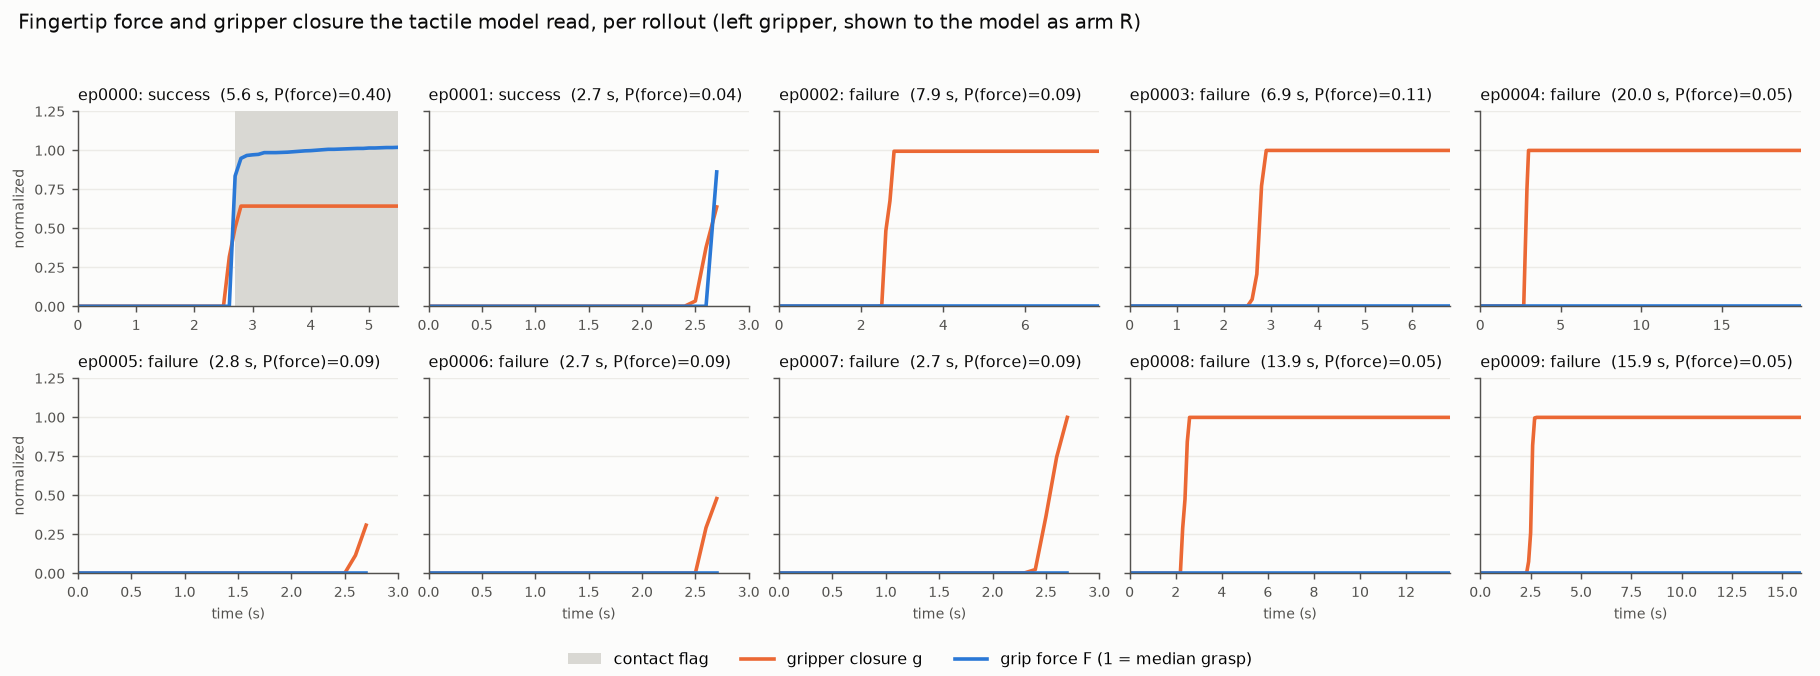
\includegraphics[width=\linewidth]{figures/force_traces.png}
  \caption{Normalized fingertip force and gripper closure for the ten Baxter rollouts. Only the
  two successes (ep0000, ep0001) show contact; ep0001's contact is a single sampled frame at the
  very end. The eight failures close fully on nothing (closure 1.0) and several then lift the
  empty gripper.}
  \label{fig:traces}
\end{figure}

\subsection{Metrics}

Accuracy is the share of clips called correctly at the 4.0 threshold on \Es. AUROC is the
probability that a random success is scored above a random failure (ties count half). MAE is on
the 0 to 100 scale of the released evaluation. For HRDexDB, paired differences are tested with
an object-level bootstrap (AUROC) and the exact McNemar test (accuracy). On Baxter, with two
successes and eight failures, AUROC is a count over 16 ordered pairs and no significance test is
attempted.

\section{Experiment process}
\label{sec:process}

The result did not come from the first attempt, and the path matters for anyone repeating it.

\paragraph{Pilot (32 train / 16 validation clips).} The first LoRA runs showed no force benefit.
An audit found the real limits: a tiny sample, labels verified only for plumbing, and force and
video clocks that had never been aligned.

\paragraph{Expanded data, naive force rendering.} With all 618 clips, aligned clocks and frozen
object-disjoint splits, both adapters were trained with the recipe above. On the 136 development
clips: video-only 82.4\% / AUROC 0.899, force 81.6\% / 0.902, shuffled force 78.7\% / 0.885.
Still no force benefit. A deep dive into the block the model had actually read found three
defects in the representation: the hand-closure sign was inverted (Inspire joint angles run 1000
open to 0 closed), so normalization had fitted ``grasp'' on open-hand frames and the scale was
37.5 raw units against contact peaks of 1{,}000 to 3{,}000, saturating every contact at the clip
maximum; per-trial resting offsets exceeded that scale, so one clip started at maximum force with
the hand open; and the contact flag fired on every nonzero reading. A classifier over the
rendered lines reached only AUROC 0.57, against 0.78 on the raw force with a per-trial tare. The
block was nearly uninformative, which is why the model ignored it.

\paragraph{Corrected representation (the model reported here).} Only the representation changed:
per-trial tare, channels ranked by peak excess, sign-corrected closure, a 5\% contact floor, the
summary line and the classifier probability. Splits, window ids, base, recipe and seed stayed
fixed. The force arm finished its 88 updates (loss 2.49 to 0.02); the matched control arm of this
run was preempted by the cluster scheduler, so the control adapter from the previous run, whose
inputs are identical, serves as the video-only comparison. The only unmeasured difference is
run-to-run training noise.

\section{Results}
\label{sec:results}

\subsection{HRDexDB}

\begin{table}[t]
  \caption{HRDexDB held-out results. Accuracy at the 4.0 threshold, AUROC, MAE on the 0 to 100
  scale, and recall per class. The two fine-tuned models differ only in the force block.}
  \label{tab:hrdexdb}
  \centering
  \small
  \begin{tabular}{llrrrrr}
    \toprule
    Split & Model & Acc. & AUROC & MAE & Succ.\ rec. & Fail.\ rec. \\
    \midrule
    dev (136) & released, video only & 66.2\% & 0.614 & 150.0 & 0.878 & 0.403 \\
     & released, video + force & 66.2\% & 0.648 & 148.5 & & \\
     & fine-tuned, video only & 82.4\% & 0.899 & 70.6 & 0.784 & 0.871 \\
     & \textbf{fine-tuned tactile} & \textbf{85.3\%} & \textbf{0.926} & \textbf{52.9} & 0.838 & 0.871 \\
     & tactile, shuffled force & 73.5\% & 0.824 & 108.8 & & \\
     & tactile, video blanked & 53.7\% & 0.775 & 120.6 & & \\
    \midrule
    test (115) & released, video only & 67.0\% & 0.593 & 143.5 & 0.768 & 0.522 \\
     & released, video + force & 70.4\% & 0.647 & 134.8 & & \\
     & fine-tuned, video only & 69.6\% & 0.733 & 121.7 & 0.725 & 0.652 \\
     & \textbf{fine-tuned tactile} & \textbf{72.2\%} & \textbf{0.800} & \textbf{97.4} & 0.797 & 0.609 \\
    \midrule
    pooled (251) & majority class & 57.0\% & 0.500 & & & \\
     & released, video only & 66.5\% & 0.600 & & & \\
     & fine-tuned, video only & 76.5\% & 0.830 & & & \\
     & \textbf{fine-tuned tactile} & \textbf{79.3\%} & \textbf{0.873} & & & \\
    \bottomrule
  \end{tabular}
\end{table}

Table~\ref{tab:hrdexdb} gives the held-out numbers. Against the released model, the tactile
fine-tune adds 12.8 accuracy points and 0.27 AUROC over the 251 pooled clips. Against the matched
video-only fine-tune, it adds 2.8 points and 0.043 AUROC, with lower MAE on both splits (52.9
against 70.6 on development, 97.4 against 121.7 on test). The tactile model's extra correct calls
are mostly successes: its success recall is higher on both splits while failure recall stays
level.

\paragraph{Statistics.} The AUROC gain over the video-only fine-tune is $+0.043$ pooled over 251
clips, object-level bootstrap 95\% interval $+0.001$ to $+0.080$, $p \approx 0.02$; per split it
is $+0.026$ on development (not significant) and $+0.067$ on test ($p \approx 0.04$). The accuracy
gain is not significant on its own: the tactile model fixes 26 clips the video-only model gets
wrong and breaks 19 it gets right (12 against 8 on development, 14 against 11 on test; exact
McNemar $p = 0.37$).

\paragraph{The model reads the force.} With shuffled blocks the tactile model drops from 85.3\% to
73.5\% on development and loses 25 paired clips while winning 9 ($p = 0.009$), landing below the
video-only fine-tune. With the video blanked it keeps AUROC 0.775 but predicts failure almost
everywhere (accuracy 53.7\%): that is the force's own signal, consistent with the force-only
probes (0.76 to 0.80). Neither channel alone explains the result; the combination does.

\begin{table}[t]
  \caption{Where the force helps. Clips are split by how sure the video-only fine-tune is: within
  0.75 of the 4.0 threshold on \Es{} (uncertain) or further (confident). Pooled over both splits.}
  \label{tab:band}
  \centering
  \small
  \begin{tabular}{lrrr}
    \toprule
    Clips & $n$ & Video-only accuracy & Tactile accuracy \\
    \midrule
    uncertain (video-only \Es{} within 0.75 of threshold) & 101 & 66.3\% & \textbf{72.3\%} \\
    confident & 150 & 83.3\% & 84.0\% \\
    \bottomrule
  \end{tabular}
\end{table}

\paragraph{Where the force helps.} Table~\ref{tab:band} splits the clips by the video-only
model's own confidence. On the 101 clips where it sits within 0.75 of the threshold, the tactile
model is 6 points more accurate; on the 150 confident clips, under 1 point (on development alone
the uncertain band is 46 clips at 71.7\% against 82.6\%). The force settles the calls the video
cannot make and leaves the confident ones alone.

\paragraph{What the wins look like.} Of the 26 clips where the tactile model is right and the
video-only model wrong, the pattern is consistent: the video-only model under-calls successes
whose hold is visually unremarkable (long, steady contact above the median force) and over-calls
failures where the hand closes convincingly on camera but the force shows a weak grip, a
re-grasp, or contact that ends early. The three largest margins are in Table~\ref{tab:wins}. The
19 clips the video-only model wins are mostly successes the tactile model scored 3.1 to 3.8, just
under the threshold, and failures with long, strong contact that force cannot distinguish from a
hold.

\begin{table}[t]
  \caption{The three held-out clips with the largest margin in favour of the tactile model.
  Scores are \Es{} out of 5; success at 4.0 or above. Force columns are read from the block the
  tactile model saw.}
  \label{tab:wins}
  \centering
  \footnotesize
  \begin{tabular}{llrrp{5.6cm}}
    \toprule
    Clip & Truth & Video-only & Tactile & What the force showed \\
    \midrule
    standing frame \#4 (test) & success & 1.27 & \textbf{4.19} & peak $2.5\times$ grasp, 16.4~s contact ending 4.5~s before clip end \\
    serving bowl \#3 (dev) & failure & 4.66 & \textbf{2.29} & $1.4\times$ grasp but only 6.7~s of contact in a 39~s clip \\
    cactus \#6 (dev) & failure & 4.19 & \textbf{1.98} & $1.8\times$ grasp, contact ends at 14.7~s of 20.2~s \\
    \bottomrule
  \end{tabular}
\end{table}

\paragraph{A stacking check.} A logistic stack of the video-only score, the tactile score and the
force-only classifier probability, fitted object-grouped on development, reaches 88.2\% / 0.928
on development and 76.5\% / 0.800 on test; the force classifier alone gets 72.8\% / 0.787 and
76.5\% / 0.777. On the harder test objects the small force classifier is competitive with both
language models on accuracy, so the tactile model does not yet fully exploit the line it is
given: the language model, not the sensor, is the bottleneck.

\subsection{Baxter rollouts}
\label{sec:baxter-results}

\begin{table}[t]
  \caption{Six conditions on the ten Baxter rollouts (two successes). Accuracy at 4.0, AUROC over
  the $2 \times 8$ success--failure pairs, MAE on the 0 to 100 scale, and the hard scores each
  condition emitted.}
  \label{tab:baxter}
  \centering
  \small
  \begin{tabular}{lrrrl}
    \toprule
    Condition & Acc. & AUROC & MAE & Hard scores given \\
    \midrule
    released FLORA, no force & 0.80 & 0.375 & 140 & 2 on all 10 \\
    released FLORA + force block & 0.80 & \textbf{1.000} & 100 & 1 on 4, 2 on 6 \\
    fine-tuned FLORA, video only & 0.80 & 0.313 & 80 & 1 on all 10 \\
    \textbf{fine-tuned tactile FLORA, real force} & 0.80 & \textbf{1.000} & 80 & 1 on all 10 \\
    tactile, shuffled force & 0.80 & 0.250 & 90 & 1 on 9, 2 on 1 \\
    tactile, force removed & 0.80 & 0.438 & 80 & 1 on all 10 \\
    force-only classifier (printed in the block) & 0.80 & 0.500 & & \\
    \bottomrule
  \end{tabular}
\end{table}

\begin{table}[t]
  \caption{Expected score \Es{} per Baxter rollout and condition. No cell reaches the 4.0
  threshold; bold marks a success scored above every failure in its column. Only the two
  force-seeing conditions do that.}
  \label{tab:baxter-eps}
  \centering
  \footnotesize
  \begin{tabular}{llrrrrrr}
    \toprule
    Episode & Label & Released & Rel.\ + force & Video-only & Tactile & Tact., shuffled & Tact., no force \\
    \midrule
    ep0000 & success & 1.91 & \textbf{2.41} & 1.34 & \textbf{2.41} & 1.03 & 1.43 \\
    ep0001 & success & 2.00 & \textbf{1.92} & 1.05 & \textbf{1.60} & 1.03 & 1.12 \\
    ep0002 & failure & 2.01 & 1.78 & 1.40 & 1.05 & 1.05 & 1.52 \\
    ep0003 & failure & 2.03 & 1.81 & 1.99 & 1.09 & 1.08 & 2.97 \\
    ep0004 & failure & 1.91 & 1.06 & 1.60 & 1.02 & 1.02 & 1.32 \\
    ep0005 & failure & 1.82 & 1.05 & 1.05 & 1.03 & 1.03 & 1.05 \\
    ep0006 & failure & 1.99 & 1.00 & 1.05 & 1.02 & 1.62 & 1.11 \\
    ep0007 & failure & 1.85 & 1.48 & 1.03 & 1.03 & 1.03 & 1.06 \\
    ep0008 & failure & 2.04 & 1.70 & 1.75 & 1.04 & 1.06 & 2.31 \\
    ep0009 & failure & 2.02 & 1.74 & 1.55 & 1.07 & 1.07 & 2.02 \\
    \bottomrule
  \end{tabular}
\end{table}

Tables~\ref{tab:baxter} and~\ref{tab:baxter-eps} give the six conditions. Every accuracy is the
majority-class 0.80: no model scores either success at or above 4.0, so the hard answers carry
nothing and the comparison lives in the ranking. There the two conditions that see the clip's own
force block rank both successes above all eight failures (AUROC 1.0), and the four that do not
rank below chance.

\begin{itemize}
  \item \textbf{ep0000, the clean grasp.} The tactile model ranks it first of ten (\Es{} 2.41).
  The video-only fine-tune ranks it sixth, below five failures; the released model eighth, and
  its rationale says the cube ``remained on the table in the final frames'' while the cube was
  20~cm in the air (Figure~\ref{fig:ep0000}). At 96 pixels the video models do not see the lift;
  the force block does.
  \item \textbf{ep0001, one contact frame at the end.} The tactile model ranks it second, above
  every failure; video-only ranks it eighth. One contact line with closure 0.64 (stopped by the
  cube) rather than 1.0 (closed on nothing) was enough.
  \item \textbf{ep0003 and ep0008, long empty lifts.} The video-only model's two highest scores
  (1.99, 1.75): the arm closes, lifts and moves exactly as in a success. The tactile model gives
  them 1.09 and 1.04; with its force block removed they jump to 2.97 and 2.31, the top of that
  column.
\end{itemize}

The tactile model's lowest success (1.60) sits 0.51 above its highest failure (1.09); the released
model with the force block also separates the classes, but by 0.11. Shuffling the blocks drops the
tactile AUROC to 0.25 and ep0000 from 2.41 to 1.03; removing them gives 0.44 with the empty lifts
on top. The force-only classifier printed in the block scores 0.5 on these clips (it ranks ep0001,
with its 0.13~s hold, last), so the robot result cannot come from that line alone. The ranking is
carried by the model reading the force text, and the direction matches HRDexDB: force helps where
the video is ambiguous, and here the video is ambiguous on every clip.

\begin{figure}[t]
  \centering
  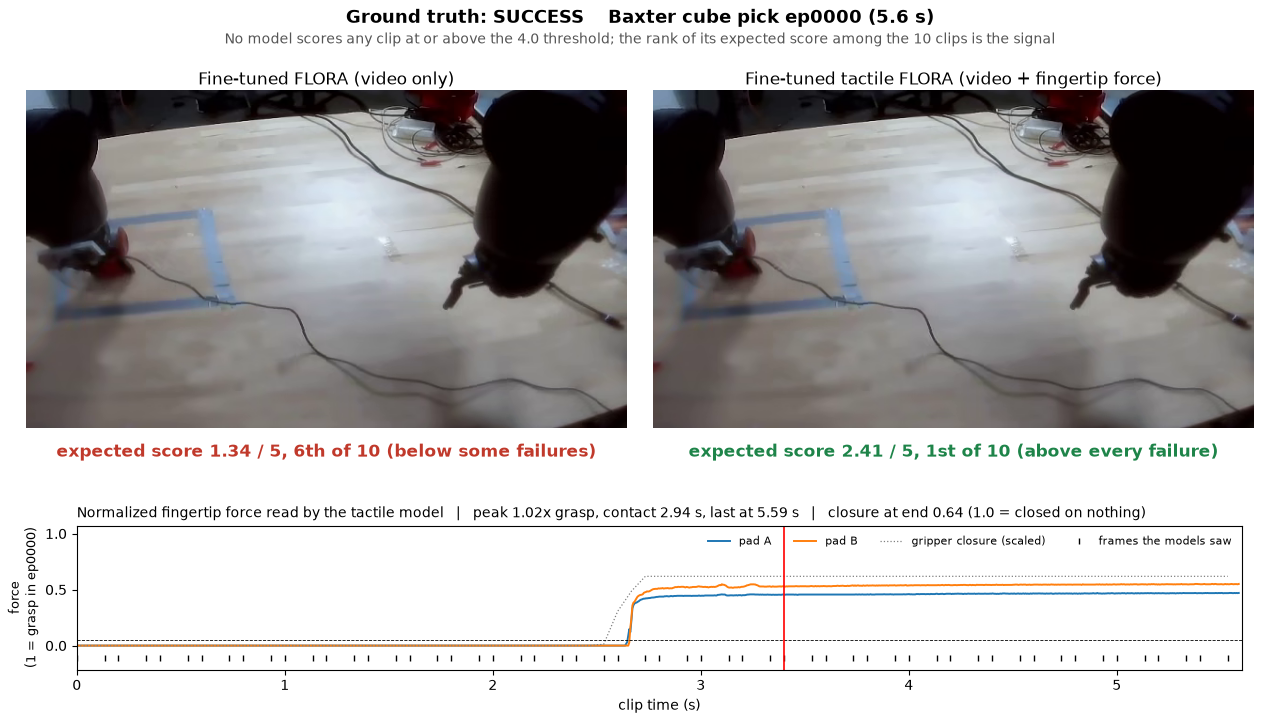
\includegraphics[width=\linewidth]{figures/ep0000_success.png}
  \caption{Frame from the side-by-side video of Baxter rollout ep0000 (success): head camera
  with each model's expected score and rank, above the normalized fingertip force the tactile
  model read. The video-only fine-tune ranks this clean grasp sixth of ten; the tactile model
  ranks it first.}
  \label{fig:ep0000}
\end{figure}

\section{Limitations}

\paragraph{Sample size.} 251 held-out clips over 32 objects cannot certify a 3-point accuracy
gain (about 1{,}000 clips would be needed at the observed win/loss ratio); the AUROC gain is the
significant one. The Baxter set has ten clips and two positives: a perfect AUROC there is 16 of 16
ordered pairs, and no significance claim is made.

\paragraph{Control provenance.} The video-only comparison is the control adapter of the previous
training run; the matched control of the final run was preempted. Its inputs are identical, so
the only unmeasured difference is run-to-run training noise, which this experiment cannot report.

\paragraph{Part of the gain rides a small classifier.} The block's summary line ends with the
probability of a gradient-boosted force classifier, and the language model reads that line as well
as the raw force lines. The frame lines and plain statistics remain in the block, and the Baxter
result cannot come from the classifier, whose own AUROC there is 0.5.

\paragraph{Undertrained.} Training loss reaches its floor by update 20 of 88 because the target is
a constant template plus one digit; both fine-tuned models are data-limited.

\paragraph{Input resolution.} Both fine-tuned models and the released baseline saw each camera as
a 96-pixel cell. The released model was trained on far larger views; higher-resolution inputs
would likely help every video model, and the force gain may shrink as the video gets stronger.

\paragraph{Baxter specifics.} Normalization was fitted on the ten test clips (label-free, but the
test set); episode 1's success rests on one line of the block; the left gripper was presented as
the right-hand pads the adapters knew; the force counts are uncalibrated.

\section{Conclusion}

Rendering fingertip force as a short text block, and fine-tuning a video reward model to read it,
improves grasp-outcome judgments on object-disjoint held-out data and transfers zero-shot to a
different robot, gripper and sensor. The gain over a matched video-only fine-tune is in ranking
($+0.043$ AUROC, $p \approx 0.02$), concentrated on the clips where video is ambiguous, and it
disappears when the blocks are shuffled. The representation is the work: the same model with a
naive rendering learned nothing. The approach needs no new architecture and keeps every input
inspectable, which makes it a practical way to add contact sensing to the reward models that are
starting to label robot data at scale. The next steps are more training clips and a second hand
to attack the data limit, calibrated fingertips and more Baxter rollouts to turn the transfer
result into a measured one, and higher-resolution video to find out how much of the force gain
survives a stronger visual channel.

\begin{ack}
We thank Rahul Chandra and the UCSD Supercomputing Club for the cluster on which every model in
this paper was fine-tuned and evaluated.
\end{ack}

\bibliographystyle{plainnat}
\bibliography{references}

\appendix

\section{Reproducibility}

All code, configurations and frozen plans are in the \texttt{tactile-flora} repository (branch
\texttt{hrdexdb-v3-force-representation}). HRDexDB: the pinned source revision, the frozen
object-disjoint split, the force configuration, the exported force classifier, the training plan
with input hashes and the Slurm job ids are recorded under \texttt{docs/experiments/}. Baxter:
the firmware, ROS node and recorder are under \texttt{tactile\_flora/baxter/}; demo collection,
dataset publishing and the rollout driver under \texttt{baxter/control/}; the ACT training scripts
under \texttt{baxter/act/}; the rollout source adapter and the preparation and evaluation
scripts under \texttt{tactile\_flora/sources/} and \texttt{scripts/cluster/}. Datasets:
\texttt{OG7407/baxter-cube-pick-left} (demonstrations), \texttt{OG7407/baxter-cube-pick-left-rollouts}
(rollouts), and \texttt{HRDexDB/HRDexDB} at revision \texttt{98b8f8e}. Side-by-side videos of
every HRDexDB clip the tactile model wins and of the Baxter rollouts, with per-clip numbers, are in
the repository's \texttt{writeup/} folder.

\section{Force-only probes on HRDexDB}

Measured before training, with object-grouped five-fold cross-validation on the 350 training
clips (majority class 68.6\%): absolute force levels and contact timing give 74.0\% accuracy and
AUROC 0.71; trial-relative hold statistics 76 to 77\% and 0.78 to 0.80; the implemented summary
line on the 64-frame grid 78.3\% and 0.78. Only 2 of 110 training failures lack contact and 100
have a contact plateau of at least 5~s, so contact timing alone cannot separate outcomes. Within
an object, successful trials hold with more force (true in 31 of 36 training objects with both
outcomes) and sustain the hold (late-over-early hold ratio 1.02 against 0.83). The exported
classifier has out-of-fold accuracy 78.3\% and AUROC 0.764 on the training clips.

\end{document}
